%% Triangles
%
% A triangle points. Pointing right or left, its index down the site leaves
% from a corner of its flat side (tn leg anchor); pointing up or down, it has
% one index on its apex side however many sites it spans (tn single). Its
% indices lean one way, in at its flat side and out at its apex, which an
% arrow on a bond follows unless the other end, or the type, says otherwise
% (tn flux).
\documentclass[border=4pt]{standalone}
\usepackage{tikz-tensors}
\begin{document}
\begin{tikzpicture}
  \tnstack{S}{3}{a}
  \tnlayer{S}{a}{tn triangle right/$A$, tn diamond/$C$, tn triangle left/$B$}
  \tnconnect[along=tn arrow]{S}
  \tnopen{down}{S}
  \tnstack[tree]{U}{2}{a}
  \tnlayer{U}{a}{tn triangle up/$U$/2}
  \tnopen{up}{U}
  \tnopen{down}{U}
  \tnstack[tree]{D}{2}{a}
  \tnlayer{D}{a}{tn triangle down/$D$/2}
  \tnopen{up}{D}
  \tnopen{down}{D}
\end{tikzpicture}
\end{document}
